\documentclass[14pt]{extbook}
\usepackage{multicol, enumerate, enumitem, hyperref, color, soul, setspace, parskip, fancyhdr} %General Packages
\usepackage{amssymb, amsthm, amsmath, bbm, latexsym, units, mathtools} %Math Packages
\everymath{\displaystyle} %All math in Display Style
% Packages with additional options
\usepackage[headsep=0.5cm,headheight=12pt, left=1 in,right= 1 in,top= 1 in,bottom= 1 in]{geometry}
\usepackage[usenames,dvipsnames]{xcolor}
\usepackage{dashrule}  % Package to use the command below to create lines between items
\newcommand{\litem}[1]{\item#1\hspace*{-1cm}\rule{\textwidth}{0.4pt}}
\pagestyle{fancy}
\lhead{Progress Quiz 4}
\chead{}
\rhead{Version C}
\lfoot{9187-5854}
\cfoot{}
\rfoot{Spring 2021}
\begin{document}

\begin{enumerate}
\litem{
Determine the domain of the function below.\[ f(x) = \frac{5}{18x^{2} +33 x + 12} \]\begin{enumerate}[label=\Alph*.]
\item \( \text{All Real numbers.} \)
\item \( \text{All Real numbers except } x = a \text{ and } x = b, \text{ where } a \in [-18.5, -17.4] \text{ and } b \in [-13.5, -11.5] \)
\item \( \text{All Real numbers except } x = a \text{ and } x = b, \text{ where } a \in [-2.2, -0.6] \text{ and } b \in [-0.7, 0] \)
\item \( \text{All Real numbers except } x = a, \text{ where } a \in [-18.5, -17.4] \)
\item \( \text{All Real numbers except } x = a, \text{ where } a \in [-2.2, -0.6] \)

\end{enumerate} }
\litem{
Choose the equation of the function graphed below.
\begin{center}
    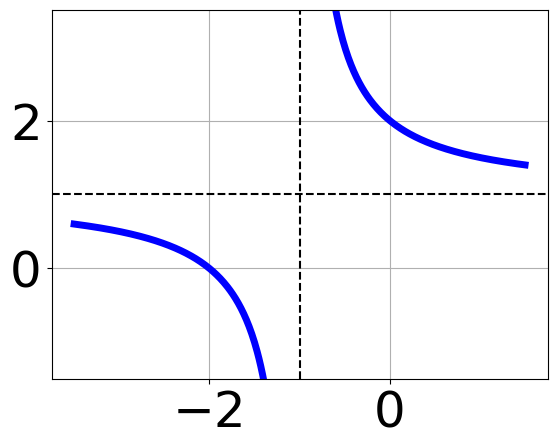
\includegraphics[width=0.5\textwidth]{../Figures/rationalGraphToEquationCopyC.png}
\end{center}
\begin{enumerate}[label=\Alph*.]
\item \( f(x) = \frac{1}{(x - 3)^2} - 5 \)
\item \( f(x) = \frac{-1}{(x + 3)^2} - 5 \)
\item \( f(x) = \frac{-1}{x + 3} - 5 \)
\item \( f(x) = \frac{1}{x - 3} - 5 \)
\item \( \text{None of the above} \)

\end{enumerate} }
\litem{
Solve the rational equation below. Then, choose the interval(s) that the solution(s) belongs to.\[ \frac{-5}{6x + 4} + 9 = \frac{-7}{-36x -24} \]\begin{enumerate}[label=\Alph*.]
\item \( x \in [-1.55,0.45] \)
\item \( x_1 \in [-0.95, -0.7] \text{ and } x_2 \in [-1.3,-0.3] \)
\item \( x_1 \in [-0.56, -0.46] \text{ and } x_2 \in [0.3,1] \)
\item \( x \in [0.72,0.9] \)
\item \( \text{All solutions lead to invalid or complex values in the equation.} \)

\end{enumerate} }
\litem{
Determine the domain of the function below.\[ f(x) = \frac{6}{30x^{2} -50 x + 20} \]\begin{enumerate}[label=\Alph*.]
\item \( \text{All Real numbers except } x = a, \text{ where } a \in [23.84, 24.07] \)
\item \( \text{All Real numbers except } x = a \text{ and } x = b, \text{ where } a \in [0.43, 0.98] \text{ and } b \in [0.99, 1.54] \)
\item \( \text{All Real numbers except } x = a, \text{ where } a \in [0.43, 0.98] \)
\item \( \text{All Real numbers except } x = a \text{ and } x = b, \text{ where } a \in [23.84, 24.07] \text{ and } b \in [24.95, 25.17] \)
\item \( \text{All Real numbers.} \)

\end{enumerate} }
\litem{
Choose the graph of the equation below.\[ f(x) = \frac{1}{x + 3} + 1 \]\begin{enumerate}[label=\Alph*.]
\begin{multicols}{2}\item 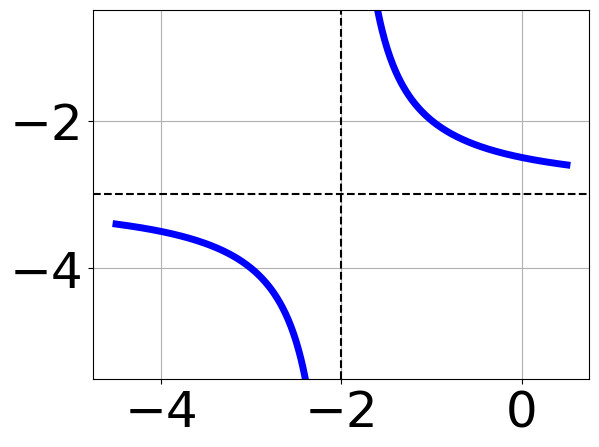
\includegraphics[width = 0.3\textwidth]{../Figures/rationalEquationToGraphCopyAC.png}\item 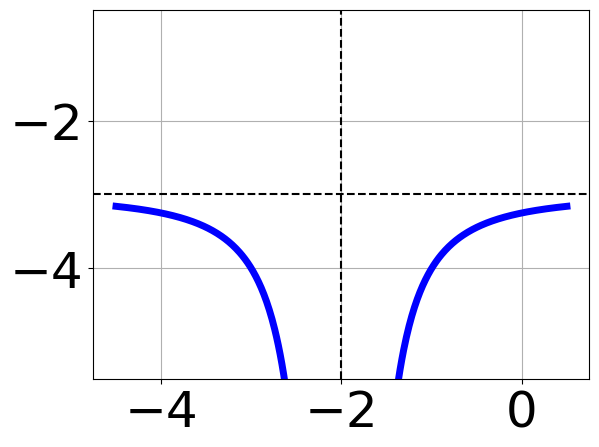
\includegraphics[width = 0.3\textwidth]{../Figures/rationalEquationToGraphCopyBC.png}\item 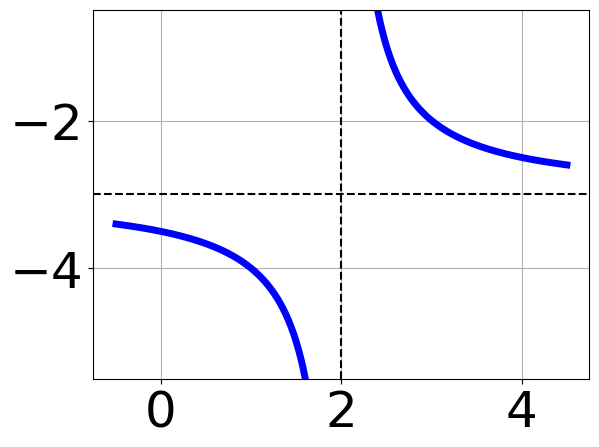
\includegraphics[width = 0.3\textwidth]{../Figures/rationalEquationToGraphCopyCC.png}\item 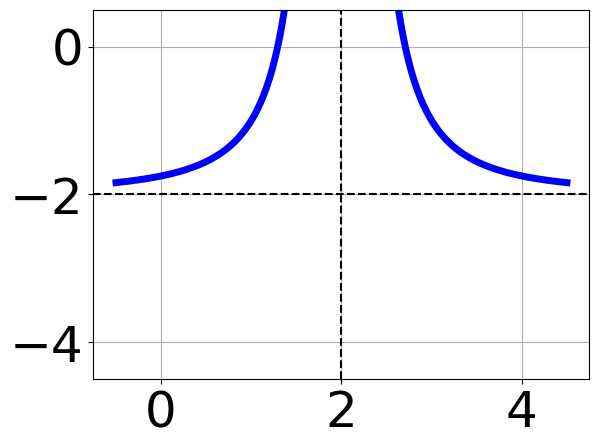
\includegraphics[width = 0.3\textwidth]{../Figures/rationalEquationToGraphCopyDC.png}\end{multicols}\item None of the above.
\end{enumerate} }
\litem{
Solve the rational equation below. Then, choose the interval(s) that the solution(s) belongs to.\[ \frac{2}{2x + 2} + -3 = \frac{-7}{-10x -10} \]\begin{enumerate}[label=\Alph*.]
\item \( x_1 \in [-1.9, 0.1] \text{ and } x_2 \in [0.3,1] \)
\item \( \text{All solutions lead to invalid or complex values in the equation.} \)
\item \( x \in [0.1,3.1] \)
\item \( x \in [-0.9,1.1] \)
\item \( x_1 \in [-1.9, 0.1] \text{ and } x_2 \in [0.9,1.8] \)

\end{enumerate} }
\litem{
Solve the rational equation below. Then, choose the interval(s) that the solution(s) belongs to.\[ \frac{-3x}{-7x + 6} + \frac{-7x^{2}}{42x^{2} -50 x + 12} = \frac{4}{-6x + 2} \]\begin{enumerate}[label=\Alph*.]
\item \( x_1 \in [0.65, 0.83] \text{ and } x_2 \in [-5.4,-0.2] \)
\item \( \text{All solutions lead to invalid or complex values in the equation.} \)
\item \( x \in [0.28,0.73] \)
\item \( x \in [-2.87,-2.56] \)
\item \( x_1 \in [0.65, 0.83] \text{ and } x_2 \in [-0.8,4.4] \)

\end{enumerate} }
\litem{
Choose the equation of the function graphed below.
\begin{center}
    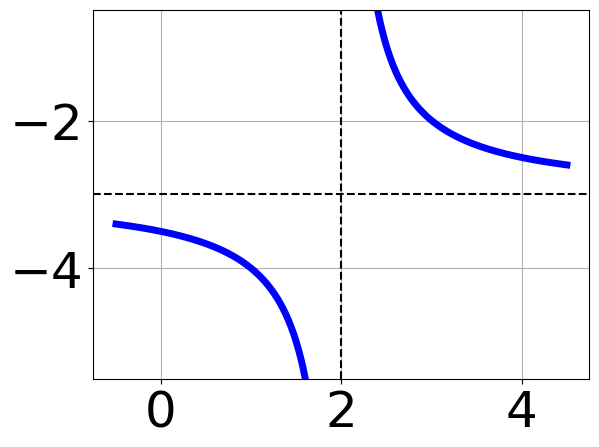
\includegraphics[width=0.5\textwidth]{../Figures/rationalGraphToEquationC.png}
\end{center}
\begin{enumerate}[label=\Alph*.]
\item \( f(x) = \frac{-1}{(x + 2)^2} - 2 \)
\item \( f(x) = \frac{-1}{x + 2} - 2 \)
\item \( f(x) = \frac{1}{x - 2} - 2 \)
\item \( f(x) = \frac{1}{(x - 2)^2} - 2 \)
\item \( \text{None of the above} \)

\end{enumerate} }
\litem{
Choose the graph of the equation below.\[ f(x) = \frac{1}{(x - 1)^2} - 3 \]\begin{enumerate}[label=\Alph*.]
\begin{multicols}{2}\item 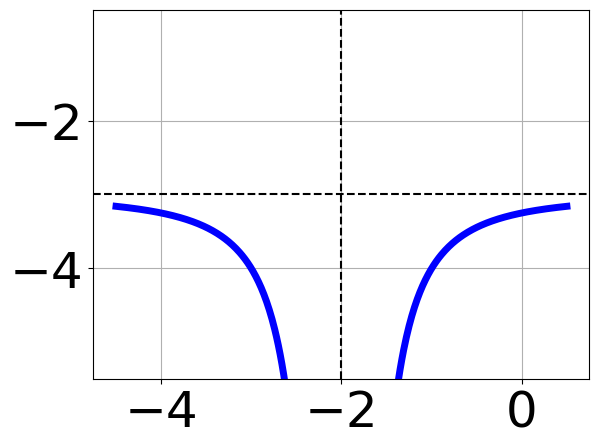
\includegraphics[width = 0.3\textwidth]{../Figures/rationalEquationToGraphAC.png}\item 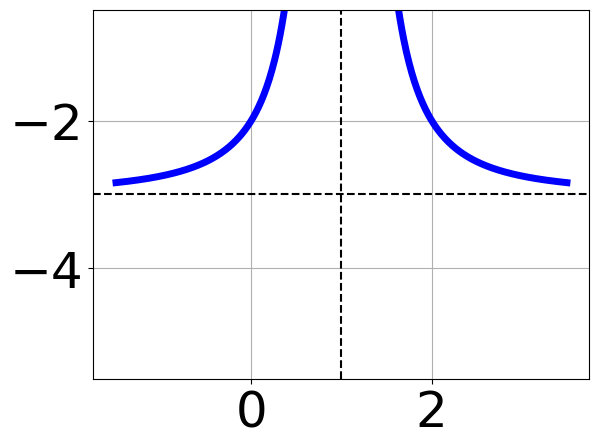
\includegraphics[width = 0.3\textwidth]{../Figures/rationalEquationToGraphBC.png}\item 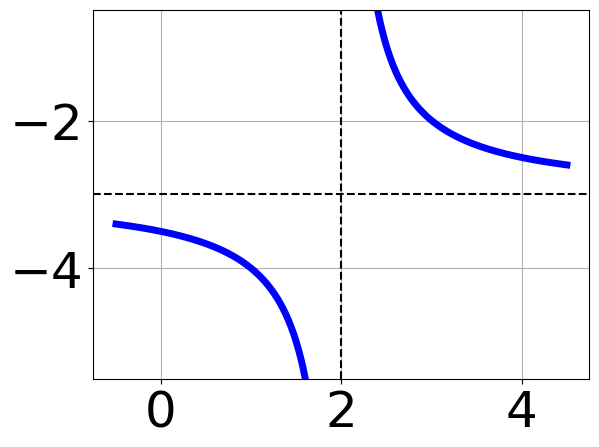
\includegraphics[width = 0.3\textwidth]{../Figures/rationalEquationToGraphCC.png}\item 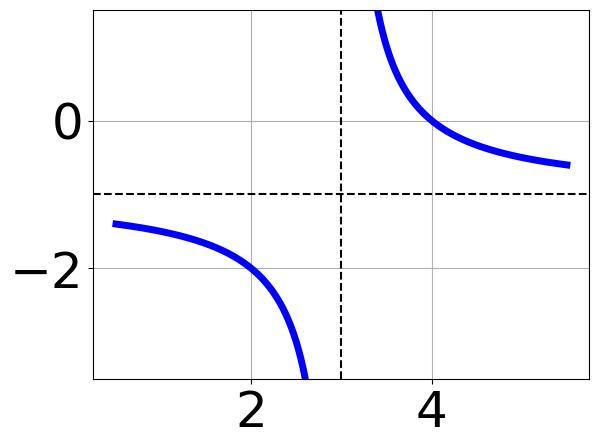
\includegraphics[width = 0.3\textwidth]{../Figures/rationalEquationToGraphDC.png}\end{multicols}\item None of the above.
\end{enumerate} }
\litem{
Solve the rational equation below. Then, choose the interval(s) that the solution(s) belongs to.\[ \frac{-2x}{6x + 6} + \frac{-3x^{2}}{-42x^{2} -60 x -18} = \frac{7}{-7x -3} \]\begin{enumerate}[label=\Alph*.]
\item \( x_1 \in [-1.06, -0.52] \text{ and } x_2 \in [3.18,10.18] \)
\item \( x \in [4.09,4.55] \)
\item \( \text{All solutions lead to invalid or complex values in the equation.} \)
\item \( x_1 \in [-1.06, -0.52] \text{ and } x_2 \in [-4,4] \)
\item \( x \in [-0.59,-0.39] \)

\end{enumerate} }
\end{enumerate}

\end{document}